\chapter{SIFT and feature matching}
In this tutorial we'll look at how to compare images to each other. Specifically, we'll use a
popular \textbf{local feature descriptor} called \textbf{SIFT} to extract some \emph{interesting points} 
from images and describe them in a standard way. Once we have these local features and their 
descriptions, we can match local features to each other and therefore compare images to each 
other, or find a visual query image within a target image, as we will do in this tutorial.

Firstly, lets load up a couple of images. Here we have a magazine and a scene containing the 
magazine:
\begin{lstlisting}[language=java]
MBFImage query = ImageUtilities.readMBF(new 
                             URL("http://dl.dropbox.com/u/8705593/query.jpg"));
\end{lstlisting}
\marginpar{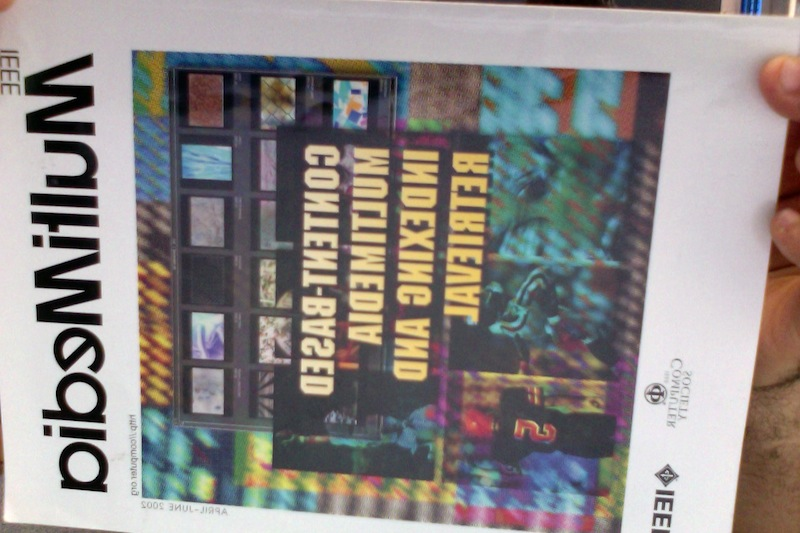
\includegraphics[width=\marginparwidth]{query.jpg}}
\begin{lstlisting}[language=java]
MBFImage target = ImageUtilities.readMBF(new 
                             URL("http://dl.dropbox.com/u/8705593/target.jpg"));
\end{lstlisting}
\marginpar{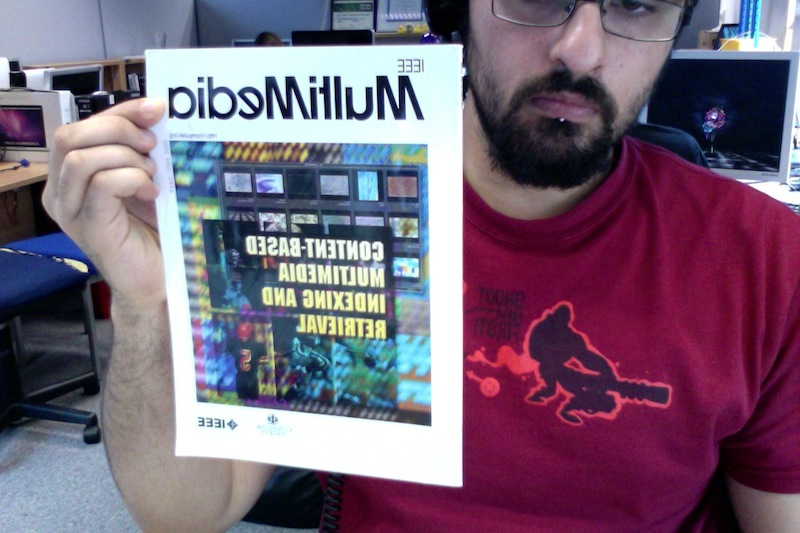
\includegraphics[width=\marginparwidth]{target.jpg}}

The first step is feature extraction. We'll use the \textbf{difference-of-Gaussian} feature detector 
which we describe with a \textbf{SIFT descriptor}. The features we find are described in a way which 
makes them invariant to size changes, rotation and position. These are quite powerful features and 
are used in a variety of tasks. The standard implementation of SIFT in OpenIMAJ can be found in the 
\verb+DoGSIFTEngine+ class:
\begin{lstlisting}[language=java]
DoGSIFTEngine engine = new DoGSIFTEngine();	
LocalFeatureList<Keypoint> queryKeypoints = engine.findFeatures(query.flatten());
LocalFeatureList<Keypoint> targetKeypoints = engine.findFeatures(target.flatten());
\end{lstlisting}
Once the engine is constructed, we can use it to extract \verb+Keypoint+ objects from our images. 
The \verb+Keypoint+ class contain a public field called \verb+ivec+ which, in the case
of a standard SIFT descriptor is a 128 dimensional description of a patch of pixels around a 
detected point. Various distance measures can be used to compare \verb+Keypoint+s to \verb+Keypoint+s.

The challenge in comparing \verb+Keypoint+s is trying to figure out which \verb+Keypoint+s match 
between \verb+Keypoint+s from some query image and those from some target. The most basic approach 
is to take a given \verb+Keypoint+ in the query and find the \verb+Keypoint+ that is closest in the 
target. A minor improvement on top of this is to disregard those points which match well with MANY
other points in the target. Such point are considered non-descriptive. Matching can be achieved in 
OpenIMAJ using the \verb+BasicMatcher+. Next we'll construct and setup such a matcher:
\begin{lstlisting}[language=java]
LocalFeatureMatcher<Keypoint> matcher = new BasicMatcher<Keypoint>(80);
matcher.setModelFeatures(queryKeypoints);
matcher.findMatches(targetKeypoints);
\end{lstlisting}
We can now draw the matches between these two images found with this basic matcher using the 
\verb+MatchingUtilities+ class:
\begin{lstlisting}[language=java]
MBFImage basicMatches = MatchingUtilities.drawMatches(query, target, matcher.getMatches(), RGBColour.RED);
DisplayUtilities.display(basicMatches);
\end{lstlisting}
\marginpar{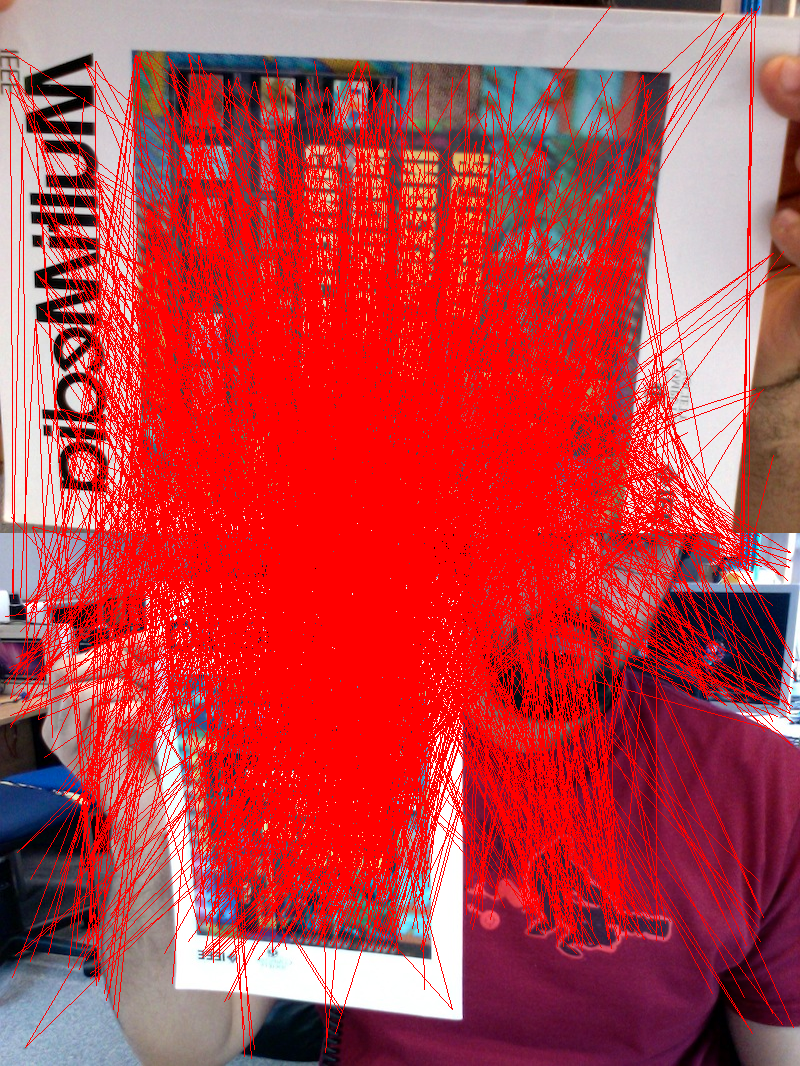
\includegraphics[width=\marginparwidth]{matches.png}}
As you can see, the basic matcher finds many matches, many of which are clearly incorrect. A more advanced 
approach is to filter the matches based on a given geometric model. One way of achieving this in OpenIMAJ 
is to use a \verb+ConsistentLocalFeatureMatcher+ which given an internal matcher, a geometric model and 
a model fitter, finds which matches given by the internal matcher are consistent with respect to the model
and are therefore likely to be correct.

To demonstrate this, we'll use an algorithm called Random Sample Consensus (RANSAC) to fit a geometric model
\marginpar{An Affine transform models the transformation between two parallelograms.}
called an \textbf{Affine transform} to the initial set of matches. This is achieved by iteratively 
selecting a random set of matches, learning a model from this random set and then testing the 
remaining matches against the learnt model. 

We'll now set up our model, our RANSAC model fitter and our consistent matcher:
\begin{lstlisting}[language=java]
AffineTransformModel fittingModel = new AffineTransformModel(5);
RANSAC<Point2d, Point2d> ransac = new RANSAC<Point2d, Point2d>(fittingModel, 1500, new RANSAC.PercentageInliersStoppingCondition(0.5), true);

matcher = new ConsistentLocalFeatureMatcher2d<Keypoint>(
  new FastBasicKeypointMatcher<Keypoint>(8), ransac);

matcher.setModelFeatures(queryKeypoints);
matcher.findMatches(targetKeypoints);
MBFImage consistentMatches = MatchingUtilities.drawMatches(query, target, matcher.getMatches(), RGBColour.RED);
\end{lstlisting}
\marginpar{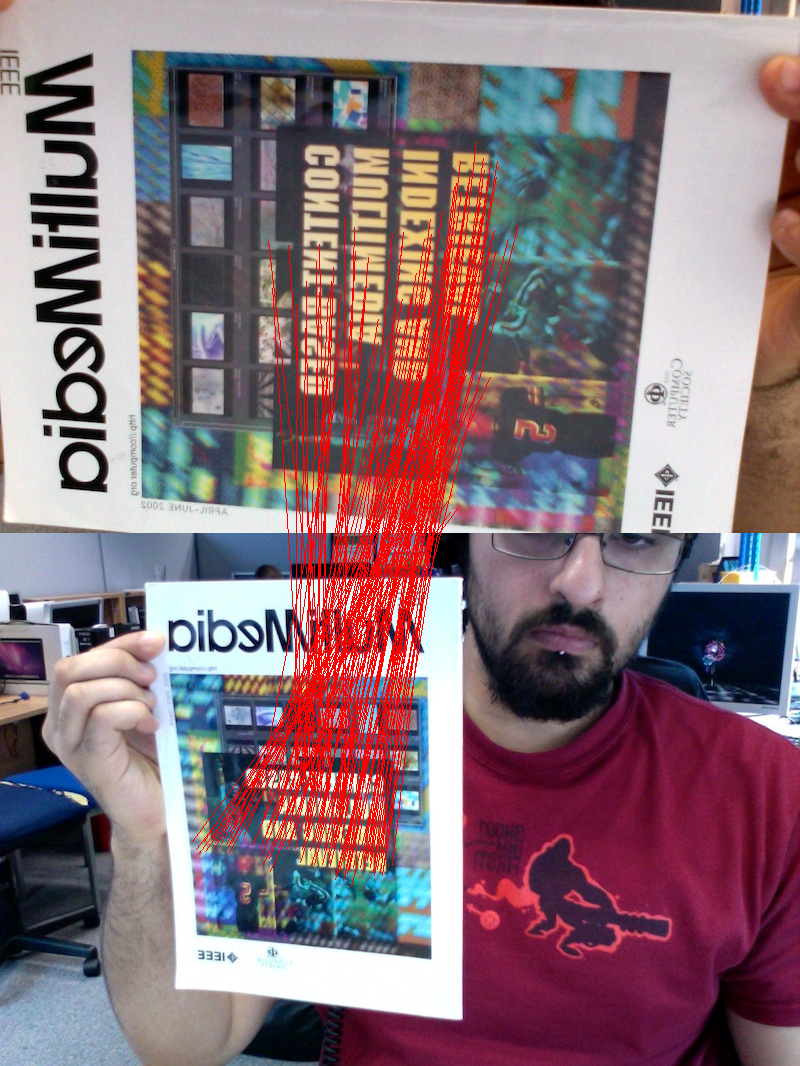
\includegraphics[width=\marginparwidth]{matches-affine.png}}
\begin{lstlisting}[language=java]
DisplayUtilities.display(consistentMatches);
\end{lstlisting}
The \verb+AffineTransformModel+ class models a two-dimensional Affine transform in OpenIMAJ. An interesting 
byproduct of this technique is that the \verb+AffineTransformModel+ contains the best transform matrix 
to go from the query to the target. We can take advantage of this by transforming the bounding box of 
our query with the transform estimated in the \verb+AffineTransformModel+, therefore we can draw a 
polygon around the estimated location of the query within the target:
\begin{lstlisting}[language=java]
target.drawShape(query.getBounds().transform(fittingModel.getTransform().inverse()), 3,RGBColour.BLUE);
DisplayUtilities.display(target); 
\end{lstlisting}
\marginpar{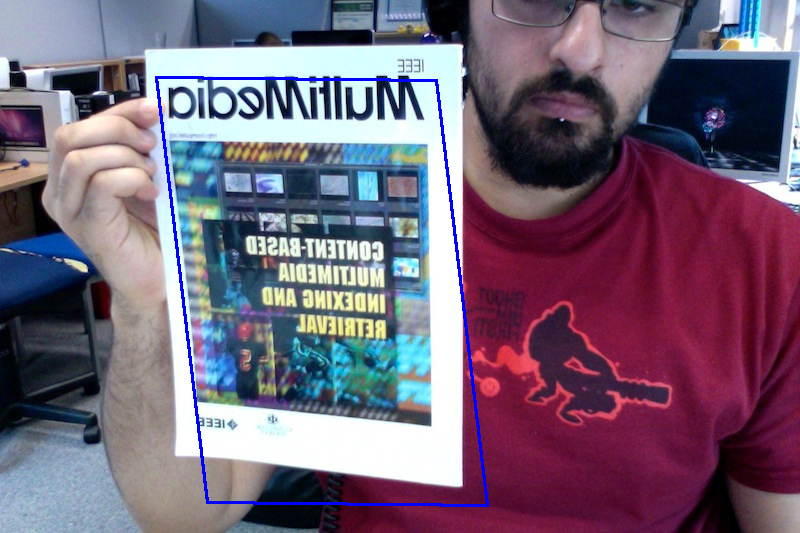
\includegraphics[width=\marginparwidth]{fittedmodel.png}}

\section*{Exercises}
\subsection*{Exercise 1: Different matchers}
Experiment with different matchers; try the \verb+BasicTwoWayMatcher+ for example.

\subsection*{Exercise 2: Different models}
Experiment \marginpar{A \texttt{HomographyModel} models a \textbf{planar Homography} between two planes. Planar
Homographies are more general than Affine transforms and map quadrilaterals to quadrilaterals.}
with different models (such as a \verb+HomographyModel+) in the consistent matcher. 

